\begin{comment}
\begin{figure*}[!h]
\begin{center}
\begin{tabular}{ll}
(2a) Categorical cross-entropy loss&(2b) Accuracy rate \\
\resizebox{.49\textwidth}{!}{
	\begin{tikzpicture} 
		\begin{axis}[
			xlabel= Epochs,
			ylabel= Loss,
			xmin = 0,
			xmax = 400,
			ymin = 0,
			ymax = .8,
			width= 100mm,
			height = 70mm,
			%legend columns=-1,
			axis x line = bottom,
			axis y line = left,
			tickwidth = 0pt,
			axis line style = { black!30 },
			legend style = {draw = none,at={(.9,.9)}, cells={anchor=west}}
			]
			\addplot+[mark=none, lila_10b, very thick,smooth] file {figures/valid/aug-max-train-loss-full.dat};
			%\addplot+[mark=none, lila_10b, very thick,smooth,dotted] file {figures/valid/noaug-max-train-loss-full.dat};				
			\addplot+[mark=none, gruen_4b, very thick,smooth] file {figures/valid/aug-max-train-loss.dat};					
			%\addplot+[mark=none, gruen_4b, very thick,smooth,dotted] file {figures/valid/noaug-max-train-loss.dat};
			\legend{ALO,SLO}
		\end{axis} 
	\end{tikzpicture}

}&
\resizebox{.49\textwidth}{!}{
	\begin{tikzpicture} 
		\begin{axis}[
			xlabel= Epochs,
			ylabel= Accuracy rate,
			xmin = 0,
			xmax = 400,
			ymin = .7,
			ymax = 1,
			width= 100mm,
			height = 70mm,
			%legend columns=-1,
			axis x line = bottom,
			axis y line = left,
			tickwidth = 0pt,
			axis line style = { black!30 },
			legend style = {draw = none, at={(0.8,0.5)},anchor=north, cells={anchor=west}}
			]
			\addplot+[mark=none, lila_10b, thick,smooth] file {figures/valid/aug-max-train-acc-full.dat};
			\addplot+[mark=none, lila_10b, thick,smooth,dashed] file {figures/valid/aug-max-val-acc-full.dat};
			\addplot+[mark=none, gruen_4b, thick,smooth] file {figures/valid/aug-max-train-acc.dat};
			\addplot+[mark=none, gruen_4b, thick,smooth,dashed] file {figures/valid/aug-max-val-acc.dat};
			\legend{ALO train,ALO validation, SLO train, SLO validation}
		\end{axis} 
	\end{tikzpicture}
	
	}\\
\end{tabular}%
\caption{Learning curves for the compared approaches. Left panel displays the the cross-entropy objective function during the learning step for the validation set. Right panel displays accuracy rate obtained on the training and validations sets during the learning step.}
\end{center}
\label{fig:learning}
\end{figure*}
\end{comment}

\section{Experiments}
\label{sec:experiments}

Experiments were conducted in the KITTI Road/Lane Dataset, part of KITTI Vision Benchmarking Suite~\cite{KITTI}. The dataset  contains  images for road and lane estimation for the task of image segmentation. It is consisted of 289 training and 290 test images. The ground-truth is manually annotated for two different road types: (i) road, road area composing all lanes; and (ii) lane, lane the vehicle is currently driving on. It is important to notice that the ground-truth is only available for training set and the test evaluation should be performed using KITTI Server.

In this work, it is used only the road ground-truths and the lane annotations were ignored. This dataset contains the same image with different ground-truths for lane and road estimation. Then, we prefer to use the road estimation and build the classifier on a binary problem~(road and background). The road type is divided in three different categories of road scenes, namely: (i) uu\_road, urban unmarked; (ii) um\_road, urban marked; and (ii) umm\_road, urban multiple marked lanes.  

{\color{green}{Rever lista de procedimentos de data augmentation}}

To increase the number of images in the training set, it is performed some data augmentation procedures. It was added images with pepper/salt noise, horizontal flipping (mirror) and  changes in contrast and brightness. Procedures that would create aberrations, such as the road in the sky and distortions that would change the nature of the objects in the scene, such as cars and pedestrians were avoided. Augmentation procedures resulted in 2601 images, divided in 2080 samples for training and 521 samples for validation (about 20\%). 


\subsection{Experimental setup}
   
Our network were build using using Keras \cite{chollet2015keras} with Tensorflow \cite{tensorflow2015-whitepaper} and trained for 100 epochs. We used a pre-trained VGG16 model to initialize the weights. Also, we use SGD optimization with learning rate set to 1e-3, decay of 5e-6 and momentum of 0.95. The default batch size contains 16 images. Other experiments with different values will be discussed in next sections. All training experiments were performed in GeForce GTX 1080 8GB GPU. HED and RCF projects provided custom functions to balance the number of pixels of edges from the non-edges pixels. Once our problem is not as unbalanced as the edge detection, we decided to use the  \textit{{categorical} {cross-entropy}} loss function.

For simplicity, in the remaining of this work, the network using the side outputs extracted at each stage of the VGG will be called Stage Layer Outputs~(\textbf{SLO}) and it is composed by $n=5$ side outputs. Similarly, for the side outputs extracted at each convolutional layer, it will be called All Layers Outputs~(\textbf{ALO}) and it is composed by $n=13$ side outputs. For comparison, it is also defined a network similar to VGG, with only the final output, without any side outputs, called No Side Outputs~(\textbf{NSO}).

The operations to combine side outputs are presented in the name of the methods. The merging operations \textbf{ADD}, \textbf{AVG} and \textbf{MAX} are available for both ALO and SLO methods. Once NSO does not contains side outputs, it does not contains merging strategies.

\subsection{Training results - Methods Comparison}

{\color{red}{Imagem 2 comentada. Texto mantido em vermelho para comparacao}}

{\color{red}{OLD - In Figure~2 it is presented the relevant curves obtained during the learning step for the proposed approaches. As one could see in Figure 2a, both compared approaches presents an expected loss curve and there is no significant difference between both approaches in terms of losses values, although the SLO model appears to be more stable and presents a faster decay than the ALO model}.

\color{red}{OLD - Regarding the accuracy rate, illustrated in Figure 2b, it is possible to see that the SLO model presents a better performance than the ALO model. The accuracy rate achieved by SLO was 0.974 while ALO it was 0.963 on the validation set (about 1.2\% worse). It is also possible to notice that the gap between the accuracy achieved in the training set and the accuracy achieved in validations set is smaller for the SLO model, which indicates that the ALO model is more prone to over-fit the data}. 

\color{red}{OLD - For the performance regarding time the average to process SLO model is 12.2\% smaller than the ALO network, and could process 33.60 images per second in training time, while the ALO model process 29.48 images per second}.}

In Figures \ref{fig:validation_loss}, \ref{fig:validation_accuracy} and \ref{fig:pixel_error} are presented the relevant curves obtained during the learning step for the proposed approaches. As one could see in Figure \ref{fig:validation_loss}, the compared approaches presents an expected loss curve and some differences for the tested approaches. ALO procedures mode appears to be more stable with a faster decay than all SLO and NSO approaches. Also, NSO and SLO approaches produces some high peaks in the learning process.

In summary, for all the metrics in the leaning step, the ALO model presented a slighted superior and more desirable behavior than the SLO and NSO models. It is believed that these results are consequence of the considerably larger amount of side outputs in the ALO model, which create more possibilities of interchangeability between confidant values.

Evaluating only ALO outputs, its is possible to see that AVG had the better performance, followed by MAX and ADD operations. The results are also more stable, but slightely close of other methods.

Figures \ref{fig:validation_accuracy} and \ref{fig:pixel_error} presents metrics the best values. Validation accuracy is related to categorical cross entropy method. The value follows the inverse behavior for categorical cross entropy loss. For other way, Figure \ref{fig:pixel_error} shows the behaviour of the methods using Fuse Pixel Error methods. It is important to see that this image indicates that SLO-MAX neural network seens to overfitting around 40 epochs. This behaviour is ignored by the other graphs. 

\subsection{Best results}

In order to improve the results a new set of tests were performed using 500 training epochs. The test were performed only for the two best CNNs in the first test set. The best accuracy rate achieve after the new training procedures by the ALO-AVG model was \textbf{0.9821} and the best fuse pixel error was \textbf{0.0332}. As for the ALO-MAX model, the best accuracy and fuse pixel error were \textbf{0.9823} and \textbf{0.0372}. The behaviour of both methods are available in Figure \ref{fig:val_acc_500_epochs}.

{\color{red}{But the instable behavior persisted, in which in some epochs were close to this top accuracy but in many others the values were close to 0.86 accuracy. Some visual results are presented in Table~\ref{table:image_segmentation}}}.

{\color{green}{Adicionar informacao sobre os resultados do conjunto de testes}}

\subsection{Evaluation results and comparison with the state-of-the-art}

After the training procedure, we create a post processing step to reduce possible noises in results proposition. For this, we used the mathematical morphology operation of Opening~\cite{najman13}. This procedure removes small noises created by the foreground~(the road)in the background. We defined a set of kernels with the sizes of $5\times5$, $7\times7$, $9\times9$, $11\times11$ and $13\times13$ and applied in the images to reduce different sizes of noises. Results using this strategy are under the label \textbf{ALO-mm} and \textbf{SLO-mm}.

Reminding that the test evaluation could only be performed using KITTI Server, the metrics provided are maximum F1-measure~(MaxF), average precision~(AP), precision~(PRE), recall~(REC), false positive rate~(FPR) and false negative rate~(FNR). 

The results achieved  on the test set according to each category in the road scenes are presented in Table~\ref{tab:metrics}. As expected, the SLO model performed better then the ALO model in all almost all of the cases. Particularly when using the post processing procedure with mathematical morphology. It is also possible to notice that although the post-processing slightly improved the overall performance, it also increased the number of false negatives. This could be an indications that perhaps the applied kernel sizes are not adequate and are removing more of the foreground than the desired.   

If compared with the state-of-the-art~(anonymous submission on the KITTI Server platform), the proposed method is comparable and sometimes superior, regarding the maximum F1-measure and the recall metrics. This is due the fact that although the reported state-of-the-art on the dataset presents a superior average precision, it also almost always presents a higher rate of false positives an negatives. This indicates that the proposed methods are more precise in delineating the regions to be segmented.       

\begin{table}
 \scriptsize
 \caption{KITTI benchmark evaluation results for each category}
  \begin{tabular}{{l}{c}{c}{c}{c}{c}{c}}
  
   \multicolumn{7}{l}{\textbf{um\_road}} \\
  \hline 
    Method & MaxF & AP & PRE & REC & FPR & FNR \\
  \hline
    \textit{SLO} & 96.92\% & 87.36\% & 94.47\% & \textbf{99.49\%} & 1.13\% & \textbf{0.51\%} \\
    \textit{SLO-mm} & \textbf{97.01}\% & \textbf{87.68\%} & \textbf{94.83\%} & 99.30\% & \textbf{1.05\%} & 0.70\% \\
    \textit{ALO}  & 96.39\% & 86.81\% & 93.87\% & 99.05\% & 1.25\% & 0.95\% \\
    \textit{ALO-mm} & 96.65\% & 87.51\% & 94.64\% & 98.74\% & 1.08\% & 1.26\% \\
    \textit{State-of-the-art} & \textbf{97.05\%}& \textbf{93.53\%} &\textbf{97.18\%} &\textbf{96.92\%} &	\textbf{1.28\%} &\textbf{3.08\%} \\
  \hline
  \multicolumn{7}{c}{} \\
  
  \multicolumn{7}{l}{\textbf{umm\_road}} \\
  \hline 
    Method & MaxF & AP & PRE & REC & FPR & FNR \\
  \hline
    \textit{SLO}  & 97.57\% & 89.44\% & 96.05\% & \textbf{99.15\%} & 1.24\% & \textbf{0.85\%} \\
    \textit{SLO-mm} & \textbf{97.61\%} & \textbf{89.67\%} & \textbf{96.30\%} & 98.97\% & \textbf{1.16\%} & 1.03\% \\
    \textit{ALO}  & 97.05\% & 88.83\% & 95.37\% & 98.78\% & 1.46\% & 1.22\% \\
    \textit{ALO-mm} & 97.21\% & 89.31\% & 95.90\% & 98.56\% & 1.29\% & 1.44\% \\
    \textit{State-of-the-art} & \textbf{97.77}\%&\textbf{ 95.64\%} &\textbf{97.75\%} &\textbf{97.79\%} &	\textbf{2.48\%} &\textbf{2.21\%} \\
  \hline
  \multicolumn{7}{c}{} \\
  
  \multicolumn{7}{l}{\textbf{uu\_road}} \\
  \hline 
    Method & MaxF & AP & PRE & REC & FPR & FNR \\
  \hline
    \textit{SLO}   & 95.16\% & \textbf{85.73\%} & 92.94\% & 97.49\% & 1.16\% & 2.51\% \\
    \textit{SLO-mm}  & \textbf{95.42\%} & 86.48\% & \textbf{93.77\%} & 97.13\% & \textbf{1.01\%} & 2.87\% \\
    \textit{ALO}   & 94.70\% & 84.87\% & 92.00\% & \textbf{97.56\%} & 1.33\% & \textbf{2.44\%} \\
    \textit{ALO-mm} & 95.20\% & 86.15\% & 93.40\% & 97.08\% & 1.08\% & 2.92\% \\
    \textit{State-of-the-art} & \textbf{95.95\%}& \textbf{95.25\%} &9\textbf{5.25\%} &\textbf{95.65\%} &	\textbf{1.21\%} &\textbf{4.35\%} \\
  \hline
  \multicolumn{7}{c}{} \\
  \end{tabular} 
  \label{tab:metrics}
\end{table}


\renewcommand{\arraystretch}{1.2}
\begin{table*}
  \begin{tabular*}{1.0\linewidth}{{c}{c}{c}{c}}
  \hline 
    \multicolumn{4}{l}{\textbf{Train set}} 
  \\
  \hline 
     & \textit{um\_000067.png} & \textit{umm\_000025.png} & \textit{uu\_000009.png} 
  \\ 
    Original Images 
    & 
    \begin{minipage}{.27\textwidth}
      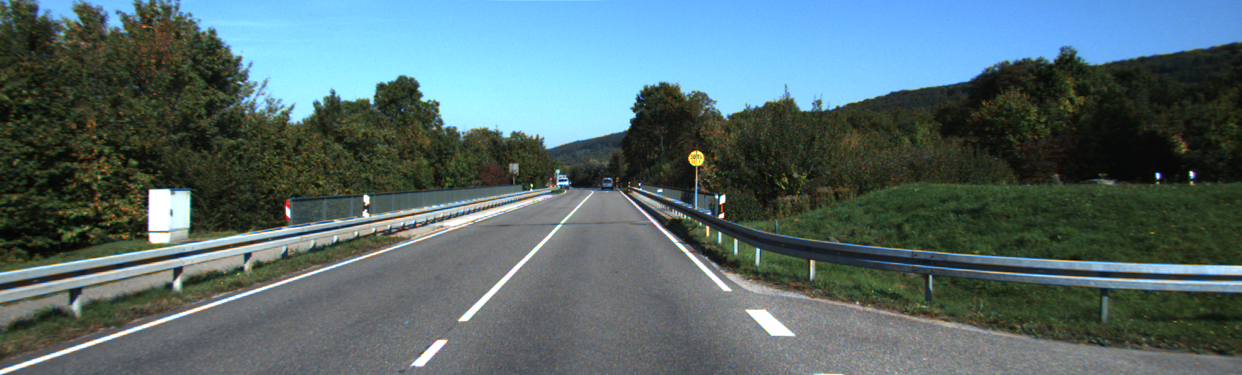
\includegraphics[width=1.0\textwidth]{figures/export/original_train/um_000067.png}
    \end{minipage}
    & 
    \begin{minipage}{.27\textwidth}
      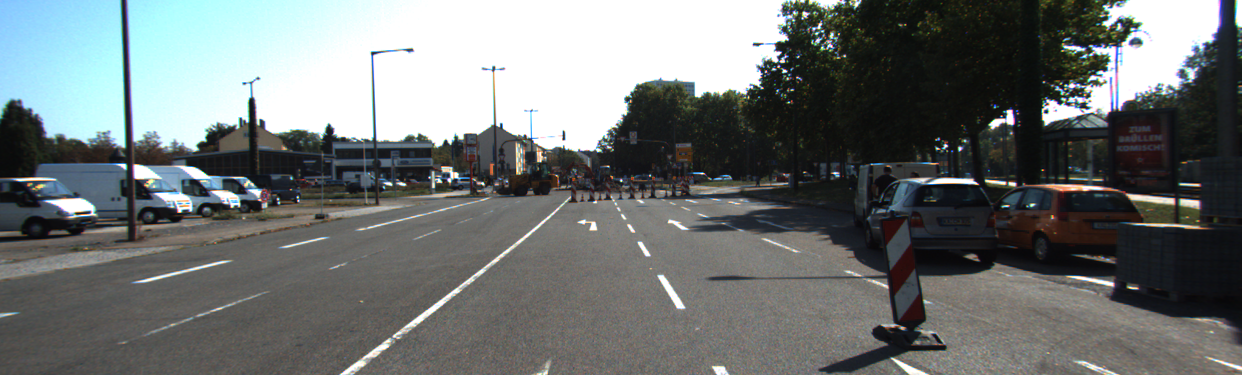
\includegraphics[width=1.0\textwidth]{figures/export/original_train/umm_000025.png}
    \end{minipage}
    & 
    \begin{minipage}{.27\textwidth}
      
\includegraphics[width=1.0\textwidth]{figures/export/original_train/uu_000009.png}
    \end{minipage} 
  \\
  \\
    ALO Marked Road 
    &
    \begin{minipage}{.27\textwidth}
      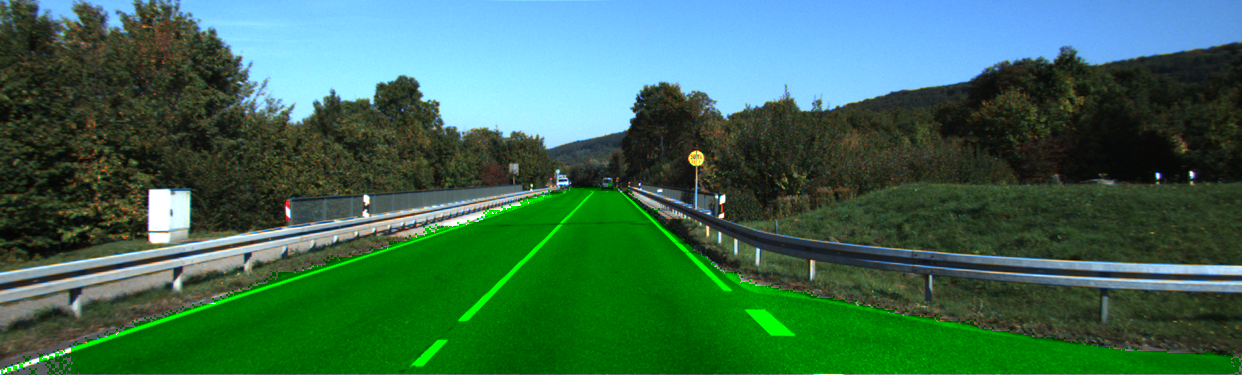
\includegraphics[width=1.0\textwidth]{figures/export/train_alo_mark/um_000067.png}
    \end{minipage}
    & 
    \begin{minipage}{.27\textwidth}
      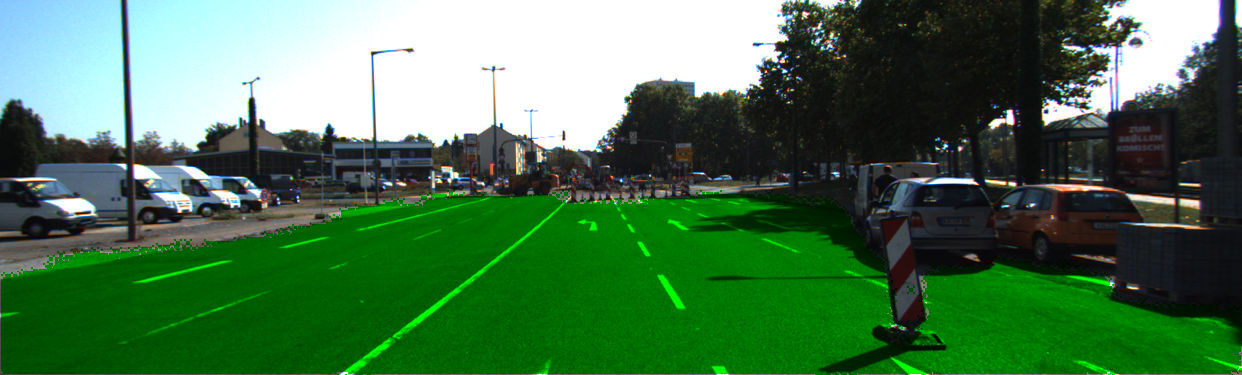
\includegraphics[width=1.0\textwidth]{figures/export/train_alo_mark/umm_000025.png}
    \end{minipage}
    & 
    \begin{minipage}{.27\textwidth}
      
\includegraphics[width=1.0\textwidth]{figures/export/train_alo_mark/uu_000009.png}
    \end{minipage}
  \\
  \\
    ALO Ground-truth 
    &
    \begin{minipage}{.27\textwidth}
      
\includegraphics[width=1.0\textwidth]{figures/export/train_alo_gt/um_000067.png}
    \end{minipage}
    & 
    \begin{minipage}{.27\textwidth}
      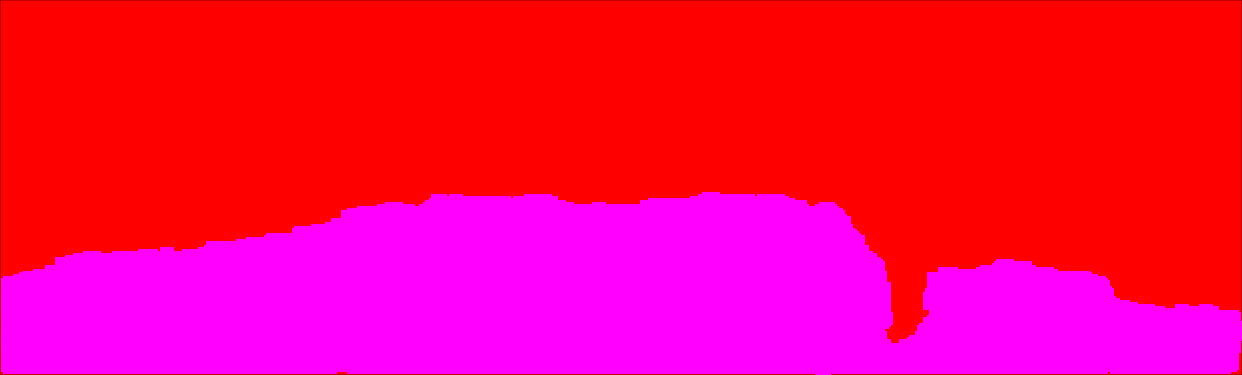
\includegraphics[width=1.0\textwidth]{figures/export/train_alo_gt/umm_000025.png}
    \end{minipage}
    & 
    \begin{minipage}{.27\textwidth}
      
\includegraphics[width=1.0\textwidth]{figures/export/train_alo_gt/uu_000009.png}
    \end{minipage}
  \\ 
  \\
    SLO Marked Road 
    &
    \begin{minipage}{.27\textwidth}
      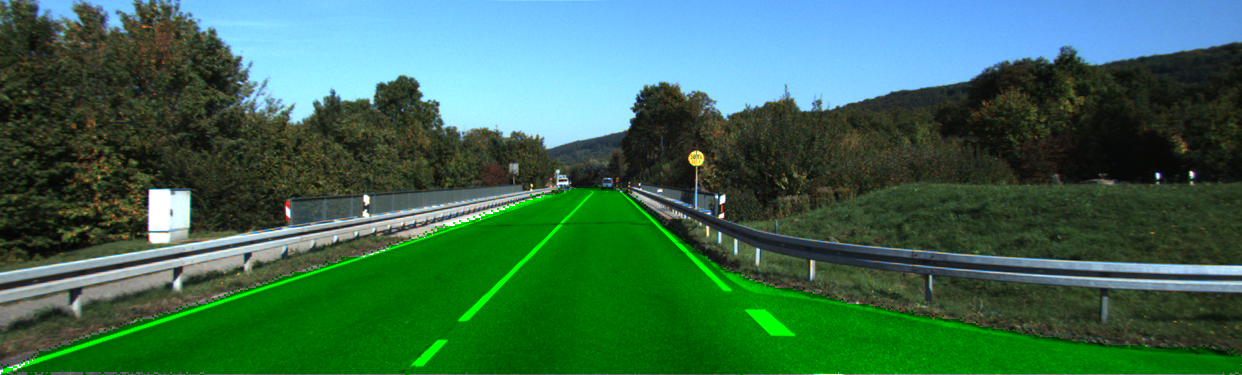
\includegraphics[width=1.0\textwidth]{figures/export/train_slo_mark/um_000067.png}
    \end{minipage}
    & 
    \begin{minipage}{.27\textwidth}
      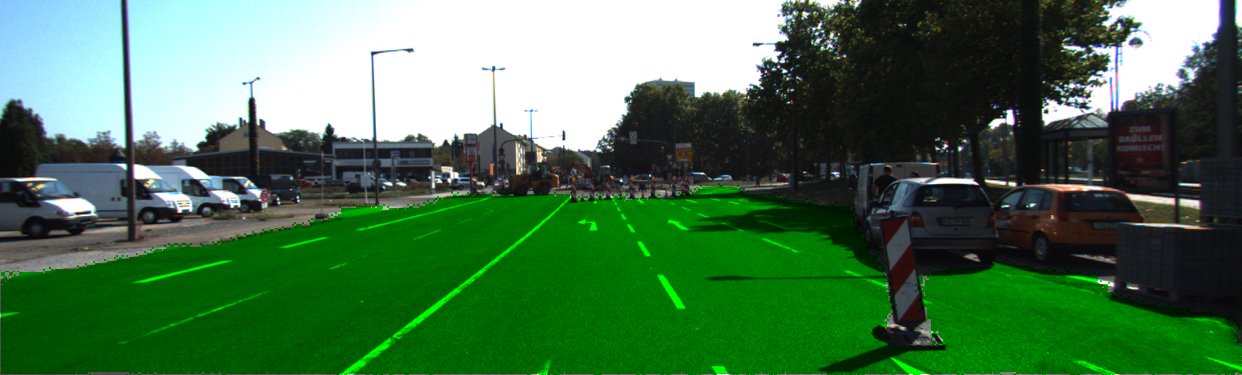
\includegraphics[width=1.0\textwidth]{figures/export/train_slo_mark/umm_000025.png}
    \end{minipage}
    & 
    \begin{minipage}{.27\textwidth}
      
\includegraphics[width=1.0\textwidth]{figures/export/train_slo_mark/uu_000009.png}
    \end{minipage}
  \\
  \\
    SLO Ground-truth 
    &
    \begin{minipage}{.27\textwidth}
      
\includegraphics[width=1.0\textwidth]{figures/export/train_slo_gt/um_000067.png}
    \end{minipage}
    & 
    \begin{minipage}{.27\textwidth}
      
\includegraphics[width=1.0\textwidth]{figures/export/train_slo_gt/umm_000025.png}
    \end{minipage}
    & 
    \begin{minipage}{.27\textwidth}
      
\includegraphics[width=1.0\textwidth]{figures/export/train_slo_gt/uu_000009.png}
    \end{minipage}
  \\
  \\
    
  \hline 
    \multicolumn{4}{l}{\textbf{Test set}} 
  \\
  \hline 
     & \textit{um\_000022.png} & \textit{umm\_000078.png} & \textit{uu\_000041.png} 
  \\ 
    Original Images 
    & 
    \begin{minipage}{.27\textwidth}
      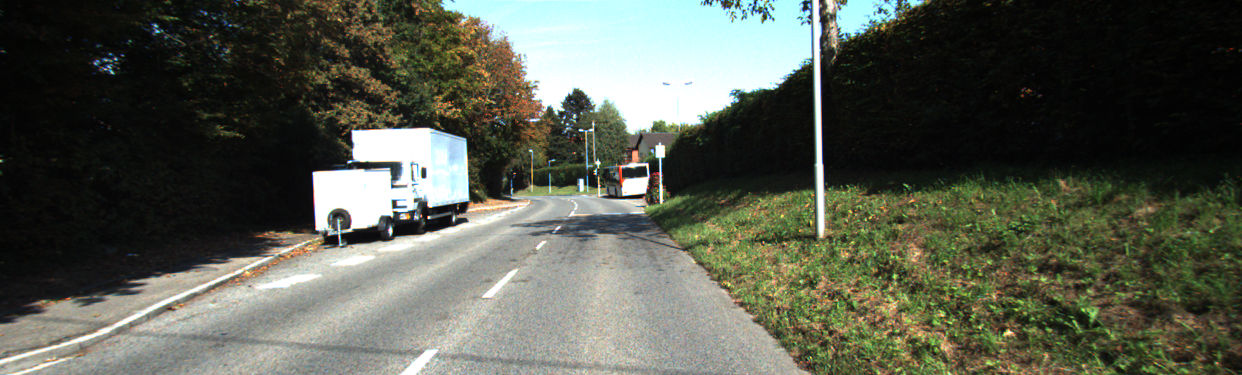
\includegraphics[width=1.0\textwidth]{figures/export/original_test/um_000022.png}
    \end{minipage}
    & 
    \begin{minipage}{.27\textwidth}
      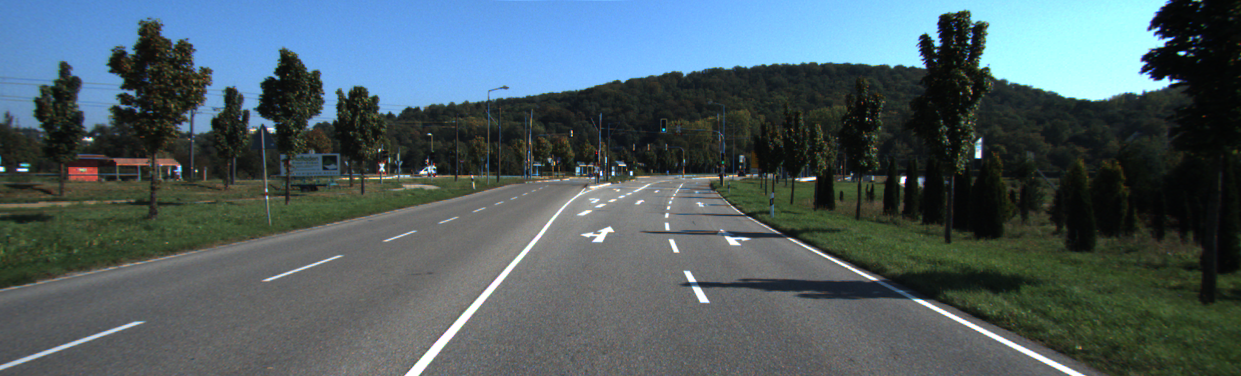
\includegraphics[width=1.0\textwidth]{figures/export/original_test/umm_000078.png}
    \end{minipage}
    & 
    \begin{minipage}{.27\textwidth}
      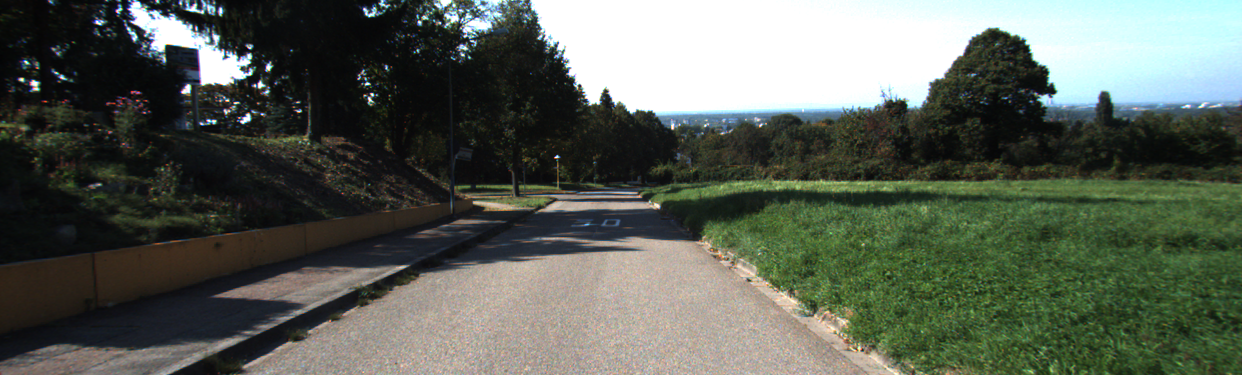
\includegraphics[width=1.0\textwidth]{figures/export/original_test/uu_000041.png}
    \end{minipage} 
  \\
  \\ 
    ALO Marked Road  
    & 
    \begin{minipage}{.27\textwidth}
      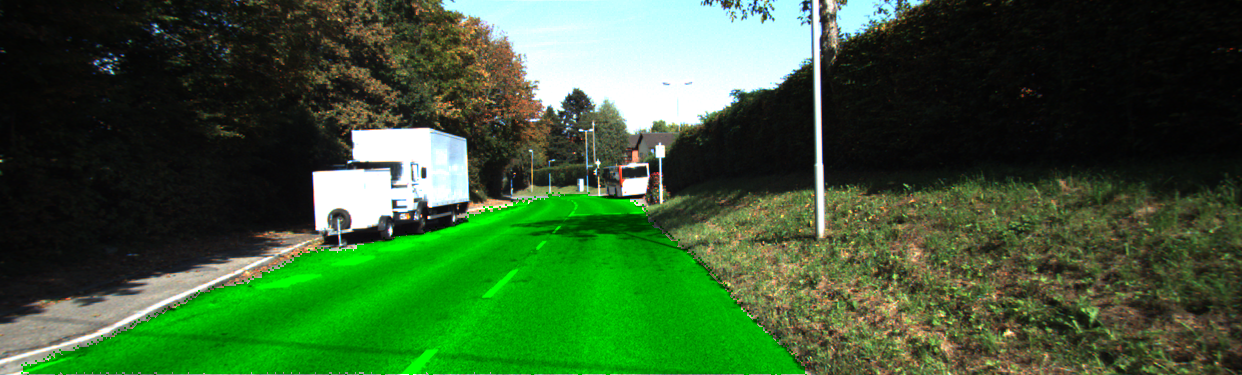
\includegraphics[width=1.0\textwidth]{figures/export/test_alo_mark/um_000022.png}
    \end{minipage}
    & 
    \begin{minipage}{.27\textwidth}
      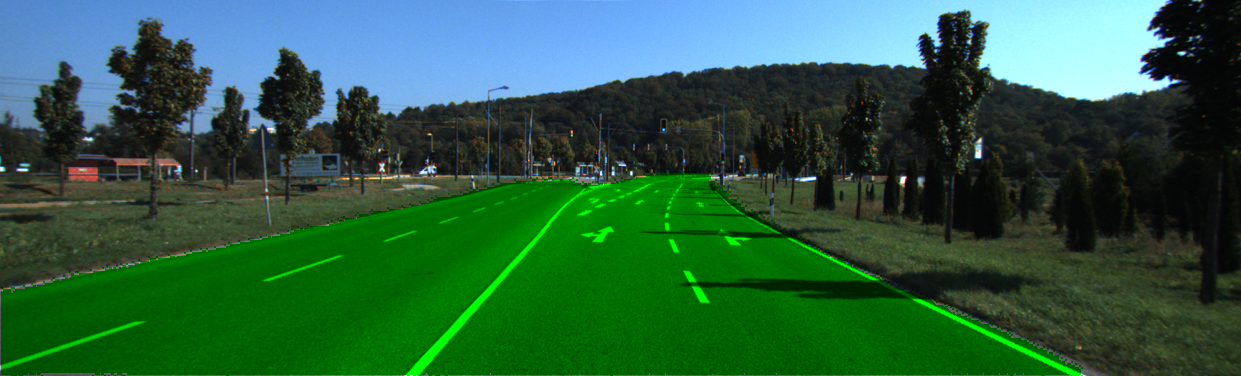
\includegraphics[width=1.0\textwidth]{figures/export/test_alo_mark/umm_000078.png}
    \end{minipage}
    & 
    \begin{minipage}{.27\textwidth}
      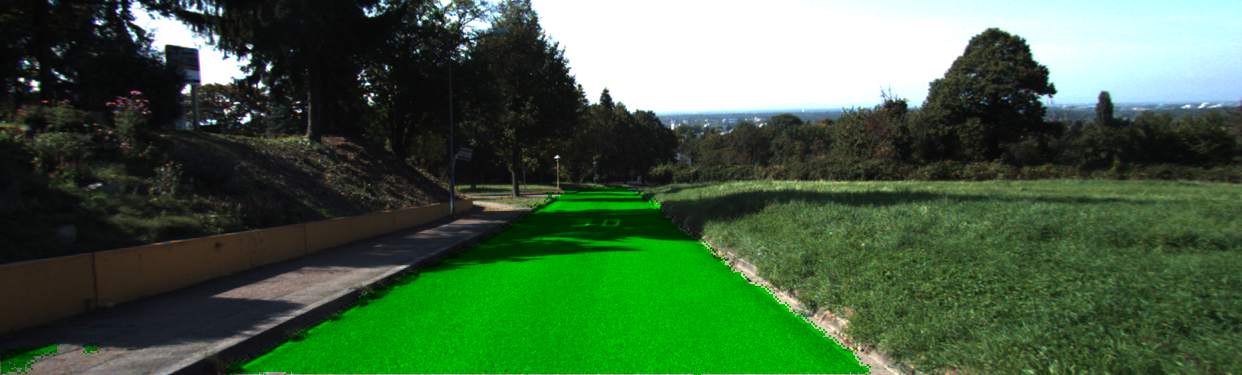
\includegraphics[width=1.0\textwidth]{figures/export/test_alo_mark/uu_000041.png}
    \end{minipage} 
  \\
  \\ 
    ALO Groud-truth  
    & 
    \begin{minipage}{.27\textwidth}
      
\includegraphics[width=1.0\textwidth]{figures/export/test_alo_gt/um_000022.png}
    \end{minipage}
    & 
    \begin{minipage}{.27\textwidth}
      
\includegraphics[width=1.0\textwidth]{figures/export/test_alo_gt/umm_000078.png}
    \end{minipage}
    & 
    \begin{minipage}{.27\textwidth}
      
\includegraphics[width=1.0\textwidth]{figures/export/test_alo_gt/uu_000041.png}
    \end{minipage}   
  \\
  \\ 
    SLO Marked Road  
    & 
    \begin{minipage}{.27\textwidth}
      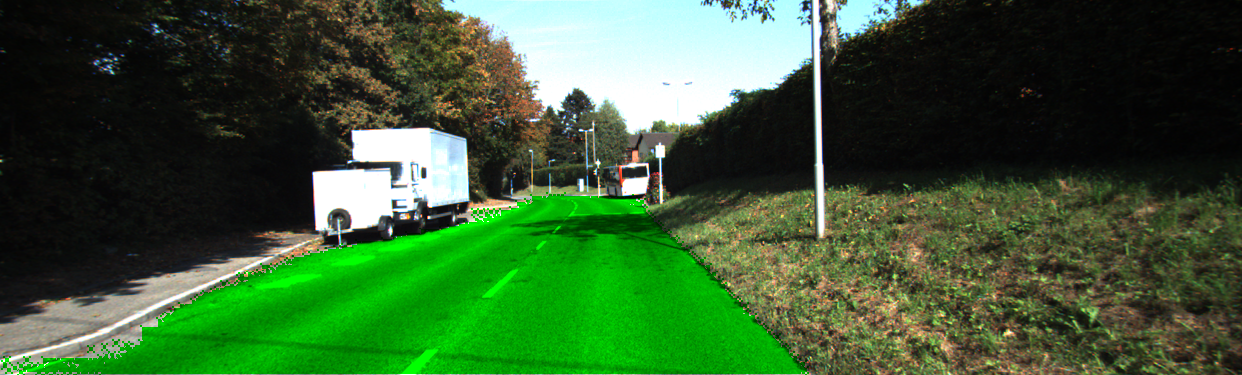
\includegraphics[width=1.0\textwidth]{figures/export/test_slo_mark/um_000022.png}
    \end{minipage}
    & 
    \begin{minipage}{.27\textwidth}
      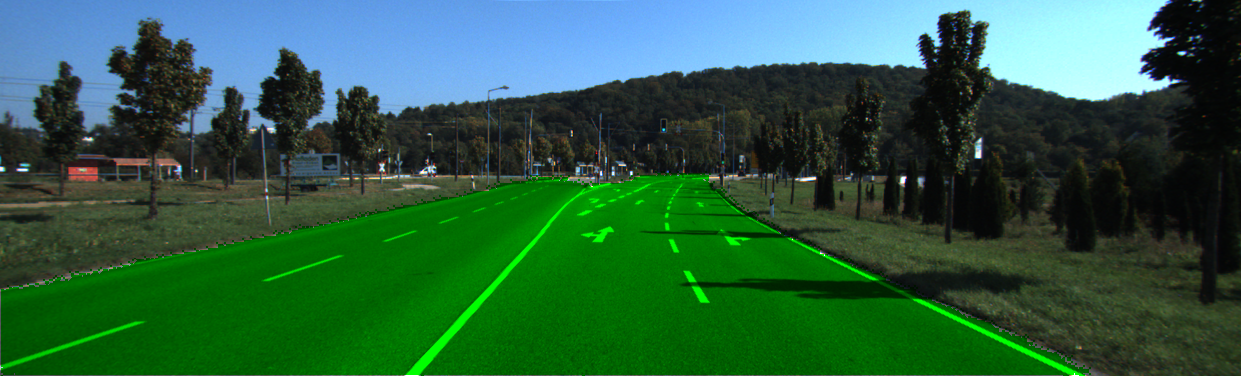
\includegraphics[width=1.0\textwidth]{figures/export/test_slo_mark/umm_000078.png}
    \end{minipage}
    & 
    \begin{minipage}{.27\textwidth}
      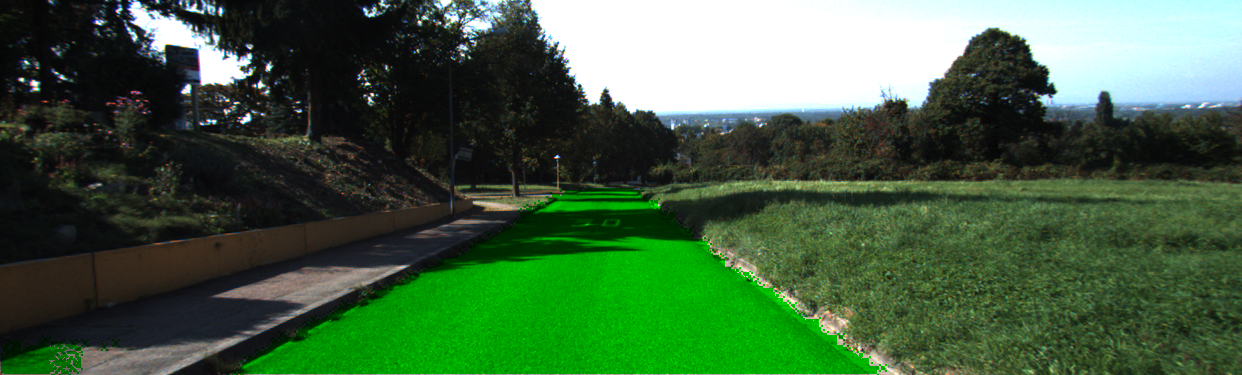
\includegraphics[width=1.0\textwidth]{figures/export/test_slo_mark/uu_000041.png}
    \end{minipage} 
  \\
  \\ 
    SLO Groud-truth  
    & 
    \begin{minipage}{.27\textwidth}
      
\includegraphics[width=1.0\textwidth]{figures/export/test_slo_gt/um_000022.png}
    \end{minipage}
    & 
    \begin{minipage}{.27\textwidth}
      
\includegraphics[width=1.0\textwidth]{figures/export/test_slo_gt/umm_000078.png}
    \end{minipage}
    & 
    \begin{minipage}{.27\textwidth}
      
\includegraphics[width=1.0\textwidth]{figures/export/test_slo_gt/uu_000041.png}
    \end{minipage} 
  \end{tabular*}
    \caption{Visual results for image segmentation}
  \label{table:image_segmentation}
\end{table*}


\begin{figure}
  \caption{Categorical Cross-Entropy Loss}
  \centering
  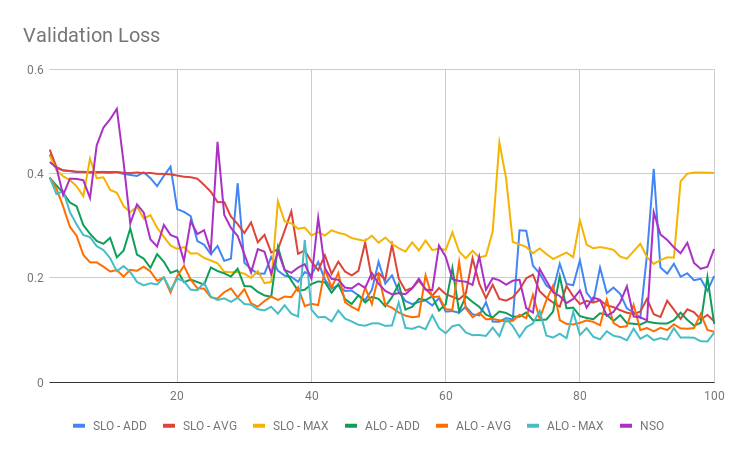
\includegraphics[width=1.\columnwidth]{figures/falreis/validation_loss.png}\label{fig:validation_loss}
\end{figure}

\begin{figure}
  \caption{Validation Accuracy}
  \centering
  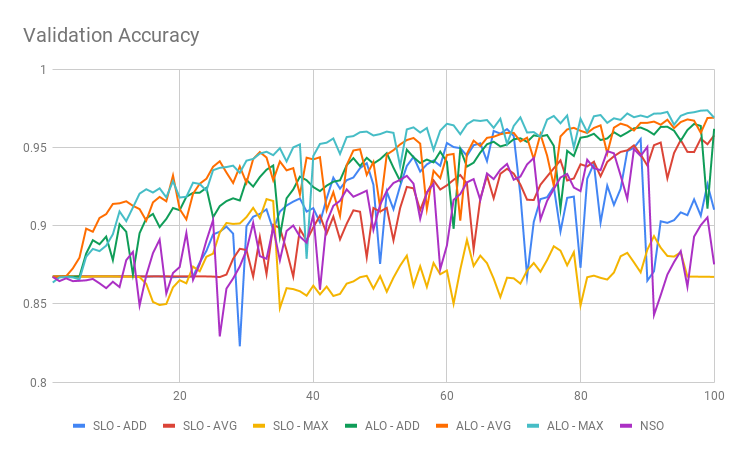
\includegraphics[width=1.\columnwidth]{figures/falreis/validation_accuracy.png}\label{fig:validation_accuracy}
\end{figure}

\begin{figure}
  \caption{Pixel Error}
  \centering
  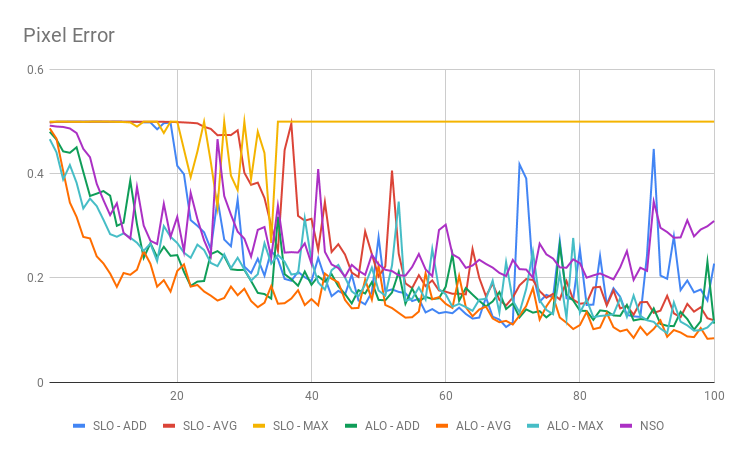
\includegraphics[width=1.\columnwidth]{figures/falreis/pixel_error.png}\label{fig:pixel_error}
\end{figure}

\begin{figure}
  \caption{Accuracy and Pixel Error for 500 epochs test set}
  \centering
  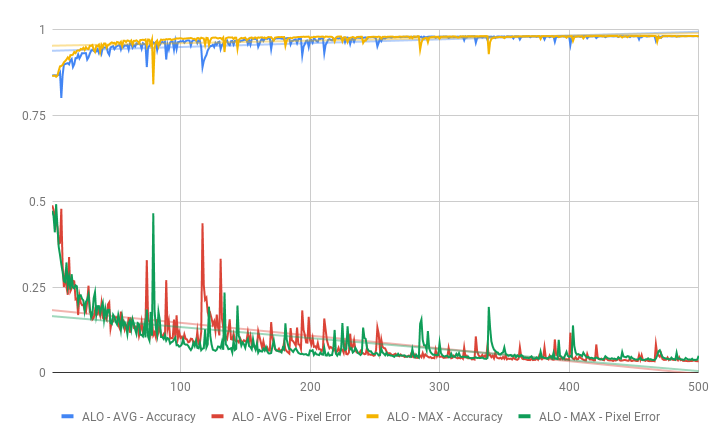
\includegraphics[width=1.\columnwidth]{figures/falreis/val_acc_500_epochs.png}\label{fig:val_acc_500_epochs}
\end{figure}




%\subsection{Post-processing using mathematical morphology}
